% !Mode:: "TeX:UTF-8" 

\BiChapter{绪论}{Introduction}\label{chap1}

%本章对 \LaTeX{} 排版系统做一个简要介绍,希望没有使用过 \LaTeX{} 的同学对 \LaTeX{} 有一个初步认识。

%=========================================================================================
\BiSection{研究背景与研究意义}{Background}\label{chap11}
%\BiSubsection{网络数据平面概述}{Motivation}\label{chap111}

%参考线性系统理论第一章的叙述方法,先要定义清楚研究对象。等等。。再看本文是否也能按照更好的方式叙述。

网络正以前所未有的速度越来越紧密地参与到民生社会中,为满足国家民生需求、新基建拉动内需和产业升级起到了至关重要的作用。从“百度一下”到网红全民直播带货,从实现“三网通”到发展“新基建”的国家战略,小到优化社会资源效率的办公数字化,大到勾勒出智能交通、智慧城市和万物互联的5G海洋,无一不是构建在网络基础设施的快速发展之上。思科公司预计,到2023年全球家用互联网总带宽将达到$5.85$Ebps\footnote{1 Ebps=$10^6$Tbps=$10^{18}$bps} (是现在的3.27倍),移动互联网用户预计达到57亿,其总流量可达$11.3$Ebps (将达到目前的5倍),其中5G流量将占据移动互联网总带宽的76.5\%(0.6\%,2019年)\citeup{huawei2019,cisco2019}。由于深度学习、AI、大数据、云计算、物联网的快速发展\citeup{gubbi2013internet,hashem2015rise},这些新技术将催使新零售、新金融、新医疗、新教育、新制造、云视频和云游戏等行业“云化”,海量的数据会在数据中心内部服务器间网络以及外部网关中传递,这些关键应用将会改变数据中心算力构成和数据中心内部网络结构特性。



近年来,网络数据平面架构的发展尤为迅速\citeup{li2019hpcc,singh2015jupiter,alizadeh2010data,wu2012tuning}。在传统网络下,为增强网络扩容能力,二层网络增加了广播、桥接等复杂功能。这种网络架构在小规模应用时可以展现强大的敏捷性与自治能力。但当网络规模进一步增加,网络中容易出现广播风暴、链路收敛慢等一系列问题。现代的大型网络设计中无需使用这类复杂的离线交互协议,事先规划好网络拓扑结构,只保留三层以上的功能,在各个层次之间的网络设备功能也逐步变得统一透明。设备统一化有助于降低网络部署的复杂度,研究人员通常需要持续进行网络测量、监控、容错、提升效能的工作。由于研究的创新和技术的推进,设备厂商不断开发出具备各种高级功能的交换芯片。硬件功能强大的同时,复杂的网络管理也遇到新的挑战。

随着云服务概念和大规模机器学习的落地,以云计算为代表的数据中心网络规模指数增长。网络功能虚拟化在数据中心内部是关键一环,虚拟交换机则是主机内各虚拟机之间数据包转发的核心软件。随着众核CPU架构快速发展,服务器内虚拟机布置资源大幅扩张,促使主机出口吞吐量从40GbE向100GbE甚至400GbE演进。不但如此,复杂的网络安全规则、流量监控等功能模块进一步吞噬了大量CPU资源。

由此可见,深入研究计算机网络通信数据平面的问题,为应对快速变革的计算网络架构发展具有重要意义。复杂化的网络架构以及快速增长的数据包吞吐容量,对网络的管理方式以及可编程的配置能力都提出了巨大挑战。本文主要围绕计算机网络可编程化问题中的处理性能增强以及可编程灵活性提升等两个子问题进行了深入分析。可编程网络由软件定义网络(Software Defined Network,SDN\citeup{mckeown2008openflow})概念引出,其将网络的分为了控制平面与数据平面。在优化数据平面处理灵活度时,又发展出了可编程数据平面的概念,即数据包协议无关处理(Programming Protocol-Independent Packet Processors,P4\citeup{p4}),其可针对不同协议数据包的处理需求,灵活地在线升级数据平面的功能,从而大大提升数据平面的可用性。针对这两大研究领域,现有的可编程网络设计领域存在以下三个主要挑战:


\begin{itemize}
	\item {\hei 网络设备核心处理资源匮乏}:为了快速处理数据包,数据平面内部一般使用特殊的运算资源来降低每个数据包的处理耗时,例如使用快速存储器或硬件查找表,而这类专用运算资源一般会耗费较大的存储资源和制造成本。作为高性能网络内设备核心资源的流表因造价高、容量小导致网络内极易产生流表溢出等现象。随着网络数据包吞吐容量以及SDN网络对流表消耗量的快速提升,核心运算资源的供需矛盾日益凸显。
	\item {\hei 全可编程网络设备性能不足}:目前实现全部的网络功能主要依赖于全可编程平台构建的数据平面,包括基于CPU的通用软件处理平台、网络处理器以及可编程逻辑器件等。但真实环境中的包处理过程非常繁琐,目前的可编程数据平面依然有着灵活性与性能之间的矛盾,全可编程平台处理效能极低,而且目前基于CPU的处理平台性能增长放缓,这也限制未来对网络功能处理能力的提升。
	\item {\hei 终端设备网络功能编程复杂}:已有的网络数据平面编程方式主要依赖于纯软件或纯硬件的全可编程平台,但CPU已经成为主机网络通信速率的瓶颈,全可编程平台拥有极高的可编程灵活性,却缺乏与之匹配的性能支持。提升系统整体处理能力,既要对软件做优化也需要对硬件做优化,对于高性能的网络功能优化工作需要进行复杂的软硬件协同设计,开发难度大、周期长。
\end{itemize}

针对以上可编程网络系统设计领域所面临的困难和挑战,需提出行之有效的解决方案以提高目前可编程网络系统的可用性。本文从网络系统的管理控制层、核心交换层以及终端接入层出发,提出了软件硬件相结合、并利用可编程硬件与传统数据平面相结合的思路来解决相应挑战。下一小节综述了国内外网络基础设施技术的演进,主要分析其技术特征和局限短板,重点关注了现阶段实际情况下SDN可编程数据平面的灵活性与性能矛盾点,以及SDN网络架构下网络设备硬件资源匮乏的现状,为本文研究工作指明了方向和意义所在。










\BiSection{网络数据平面的研究现状}{research content}\label{chap12}

近年来,网络数据平面呈现井喷式发展,对网络设备性能的提升带来极大需求以及挑战。IDC报告称,2019上半年中国公有云服务整体市场(Iaas/PaaS/SaaS)达到54.2亿美元,并预计在未来5年间内以年均复合46\%的速度快速增长\citeup{idc2019,idc2020}。数据中心内服务器计算力呈现异构化趋势,GPU,AI芯片,FPGA等使用非通用类型指令集和特殊体系架构计算单元已成为目前分布式计算领域的热点话题。现在超大型数据中心一般可容纳数十万台终端服务器,内部网络链接数量多、拓扑规模大、传送海量数据,这使得现有的网络变得异常复杂\citeup{hong2018b4,singh2015jupiter,mckeown2008openflow,casado2007ethane},同时新的数据包类型层出不穷也使传统网络显得不够灵活。

接下来本小结将简要介绍网络数据平面可编程技术背景,之后从三个方面回顾网络数据平面可编程研究的现状,分别是网络数据平面控制系统设计、网络数据平面的可编程硬件设计,以及网络数据平面的可编程抽象方法。

\BiSubsection{网络数据平面的可编程技术}{Technology Brief}\label{chap1125}

{\hei 1)软件定义网络与网络可编程概念}

为解决设备制造复杂和设备管理复杂的问题以及应对网络灵活性不足的挑战,软件定义网概念下的可编程网络思想被提出。SDN将数据平面和控制平面解耦。在数据平面上,对数据包的处理统一做查找-转发(Match-Action)抽象。控制平面负责建立网络拓扑,控制并下发流表。这样所有的数据包转发行为都由控制平面的软件逻辑管理,数据平面需要支持任意一种网络协议。由于软件具有强大的灵活性以及开发的敏捷性,SDN大大加速了网络创新和智能化管理的进程。数据平面和控制平面的通讯桥梁由符合OpenFlow协议的安全通道(Secure Channel)构成。因此数据平面统一化、简单化,使得网络交换设备向白盒化方向发展。	

\begin{figure}[!ht]
	\centering 
	\vspace{-1.5mm} 
	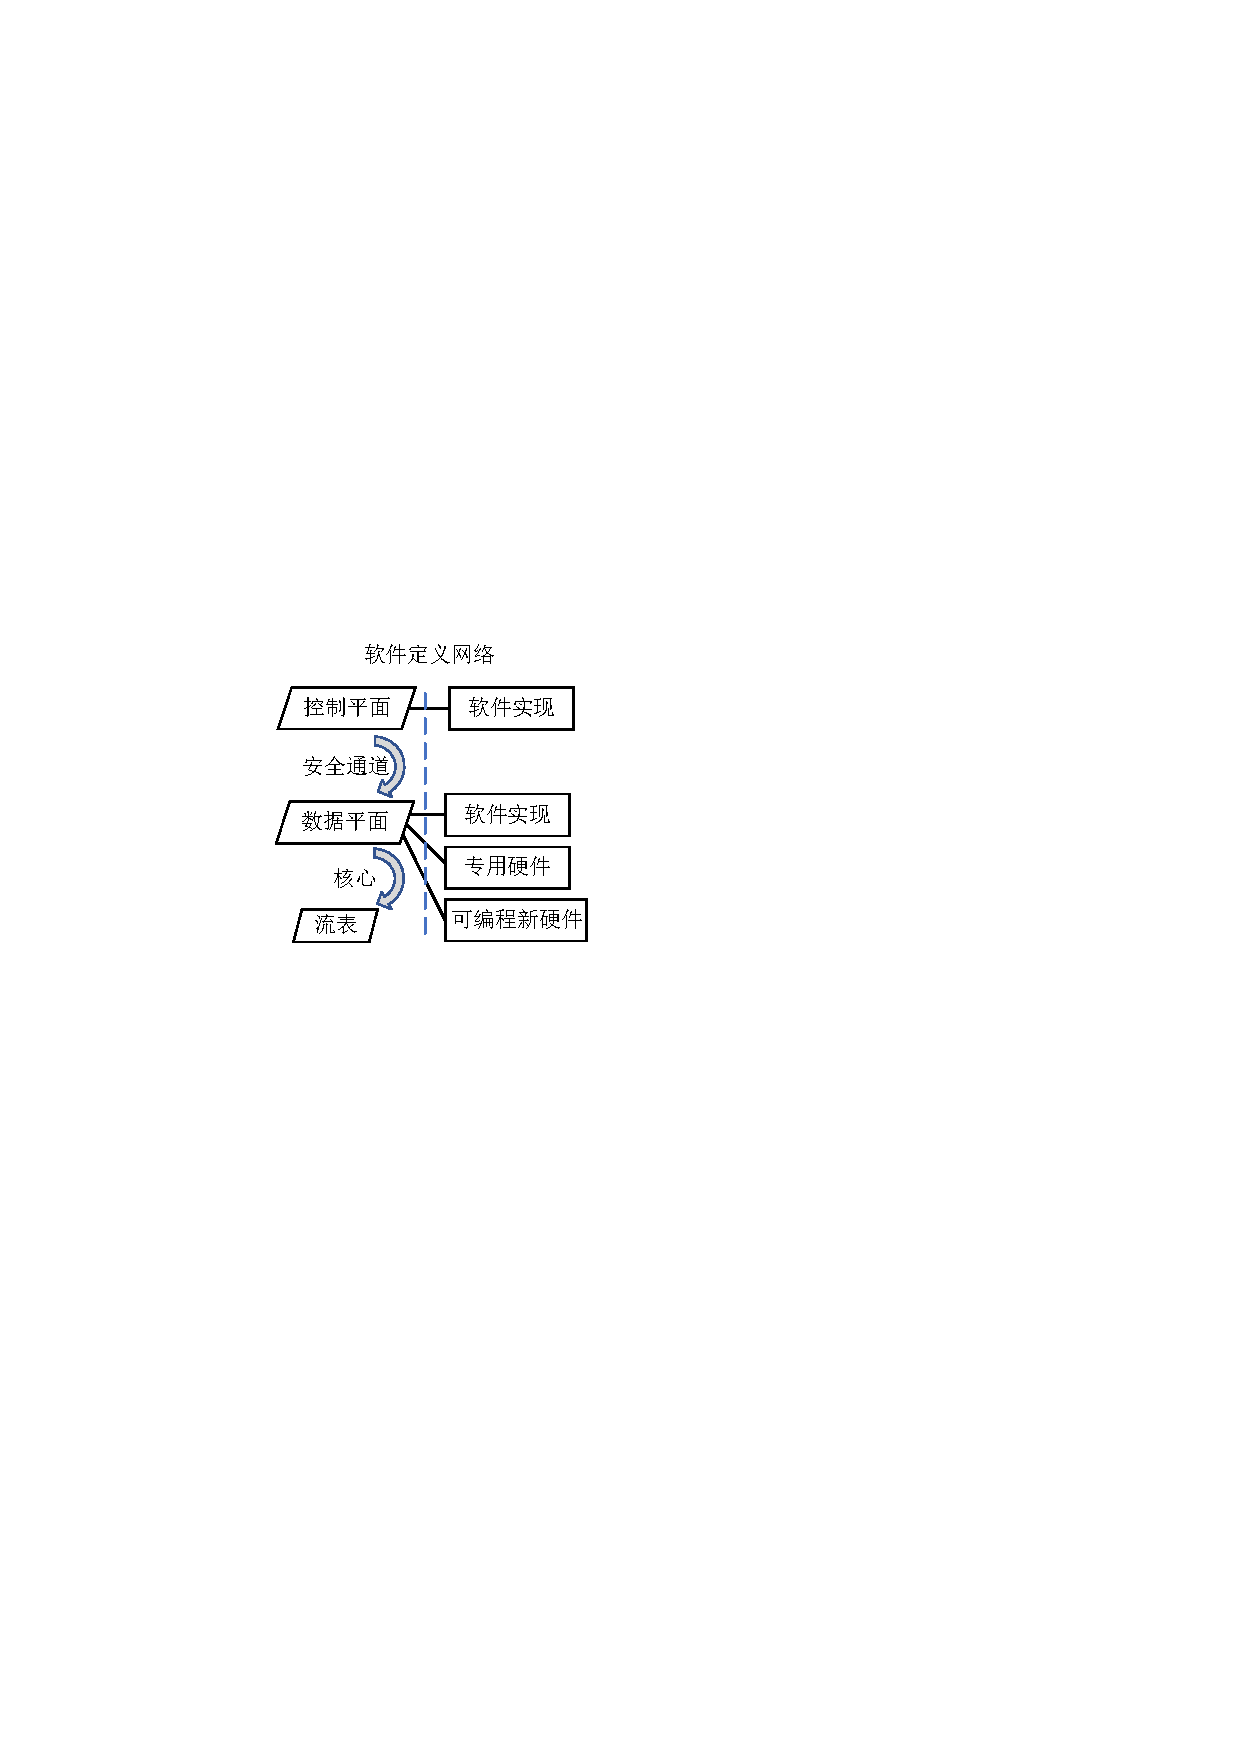
\includegraphics[scale=1]{sdnarcs.pdf}
	\caption{软件定义网络结构及其实现方案} \label{fig:sdnarcs}
\end{figure}

软件定义网络的基本设计概念是将数据平面与控制平面分离\citeup{mckeown2008openflow,ethane}。
其中网络数据平面完成计算机之间通信数据包的匹配、修改、传送、转发的软硬件设备。
数据平面的可编程性核心依赖于流表及其配置操作,网络管理员拥有对数据平面的各个特性做快速个性化定制的能力。
网络的控制平面维护全网视野、调度、配置针对流的转发条目。
运行在控制平面内的各种应用构成了其全部功能。
当前SDN网络系统设计架构如图\ref{fig:sdnarcs}所示,主要有软件方法实现,专用硬件实现和新型可编程硬件。



在不同场景下,网络对数据通信的需求千差万别,根据应用场景流量大小不同、处理过程复杂程度来设计选取数据平面的实现方案。本文在第\ref{sec:pdpintro}章详细介绍各类数据平面的实现方案的优缺点,并着重于各类数据平面可编程性的分析。目前最主要的两类数据平面是“软件交换机”和“专用硬件交换机”。两者在功能上都能够对数据包做一系列处理,包括匹配、查找、统计、传送、转发和安全校验等,其中“流表”是实现数据平面功能的核心函数(器件)。数据平面包含一个可以与远端控制器沟通的代理机构,这部分功能着重于协议通信以及安全通道信息加解密,主要由轻量级处理器构成。硬件交换机之于软件交换机的主要区别在于处理数据包的性能以及交换容量。数据包处理性能主要参数为吞吐量(字节每秒)和包吞吐量(包每秒)。目前基于软件实现的数据平面性能可达到60Gbps/60Mpps\citeup{pisces}。当数据包处理复杂度(操作步骤数量)增加时,软件交换机的性能会大幅下降。专用硬件交换机有接口数目多、交换容量大的特点,一般能满足64个100G端口的总交换容量。而且硬件交换机转发时延低,性能与数据包处理步骤数目几乎无关,稳定性良好。在核心网络和高性能网关等领域主要使用基于硬件的交换设备,但成熟设备功能固定、更换成本高,如果需要更新网络功能,几乎无所适从。所以目前在数据中心网络的NFV(网络功能虚拟化)等场景内,软件交换机依然占据很大份额。由于软件交换机灵活性高,开发人员能够快速迭代部署新功能,且传统单机通信速率需求不高,软件交换机尚能满足需求。但随着人工智能、5G领域的发展,数据中心网络内通信容量需求快速增长,转发时延收紧,软件交换机性能瓶颈凸显。运营商不得不为网络任务大量堆叠服务器。本文主要侧重于研究服务器和核心交换网络中,如何使用可编程硬件来大大缓解网络性能瓶颈。针对控制平面,本文使用SDN全局优化的思想,实现对网络中的瓶颈资源(如流表资源)的可扩展性并提升通信协议的安全性。


{\hei 2)数据平面可编程概念}

随着创新需求的进一步提高,只有让底层硬件拥有灵活的可配置能力才能满足目前行业变革的需求,因此研究人员提出了数据包处理编程协议无关(Programming Protocol-Independent Packet Processors,P4)概念。如果说SDN给出了控制层的全局视野,那么协议无关可编程的数据平面给出了设备层的全局视野。SDN已经将数据平面高度抽象,操作人员可以灵活地定义数据流,以及对这种流进行怎样的操作。但是在数据平面内数据包头的匹配域却是预先规划好的。固有转发平面的设计思想会引起如下两个问题:其一,添加新特性需要跟业界讨论、以及等待很长的设备研发时间;其二,在数据平面内固化现实中可能出现的每一个网络协议字段造成宝贵计算资源的巨大浪费。满足新阶段的网络创新需要具有比SDN概念更好的灵活性、动态性。因此斯坦福大学提出了P4\citeup{p4}编程语言框架,这种语言有能力重新定义数据平面的包解析模式。P4源代码通过前端编译器编译为中间表示层代码,这个编译过程将提出源代码中的语义逻辑。之后需要根据不同的目标器件再进行后端编译,这个过程最终会生成目标器件对应的机器码,硬件可直接读取。目前P4的目标设备已经有基于ASIC的交换芯片、CPU、GPU和FPGA等多种实现。

P4扩展了可编程抽象的灵活性,包括可编程的包头域抽取器,以及可编程的多级流表。P4同时规范了一种编程语言\citeup{p4},它可以控制数据平面对数据包的任意解析行为,也可以自由配置查找表的数据位宽和多级流表之间的查找流水线\citeup{rmt,mswitch}。这种更高阶的硬件编程模型使交换设备更加透明,设备与网络协议解绑。除此之外,网络端到端的大带宽、低时延需求引申出了网络功能硬件卸载、网络随路计算等概念,这也进一步促使网络面向全面可编程化方向发展。
协议无关处理器从诞生至今已经覆盖了广泛的网络应用场景:
1)替代传统网元(服务负载均衡\citeup{miao2017silkroad}、安全控制\citeup{lapolli2019offloading}、流量控制\citeup{yang2018elastic}、测量\citeup{kim2015band}),使云网络自身成为一个软硬任务分配均衡且可编程的系统。
2)增加网络随路专用功能,如键值查询(key-value store)\citeup{jin2017netcache}。旨利用网络高速以及可编程交换机特点,使特殊功能的性能大幅提升。

P4规范的网络可编程数据平面可编程性依然比较弱,只能自主设定包头域以及匹配表,无法增加其他适应性计算。
在一些网络延时要求严苛的场景,网络随路计算概念应运而生,网络可编程性差也成了制约网络发展的关键因素。
编程灵活性,与吞吐性能是天平的两端,由于网络巨大的性能需求,很难同时获得很高的可编程性。在此之外,也有很多特性是P4架构无法实现的:
1)包头长度有限,目前数据平面可编程的流水仅仅紧局限于处理宽度受限的包头。
2)非图灵完全,只有有限个数的固化的“执行器”。
3)没有讨论包调度问题。
4)无法对数据包进行可编程的带状态处理。而这些问题目前被认为是因追求高性能而带来的设计折中\citeup{lec8rmtp4,chole2017drmt}。






\BiSubsection{网络数据平面控制系统设计}{Application and research status}\label{chap121}

{\hei 1)软件定义网络数据平面的控制系统}


软件定义网络(Software Defined Networking,SDN)\citeup{mckeown2008openflow}的诸多优势是由于网络结构逻辑分层带来的。SDN将控制平面抽离出来,形成对网络分布式数据平面的集中控制的结构。作为控制平面与数据平面交换机通信接口OpenFlow协议是目前最具影响力的,已经成为了业内事实标准。SDN将网络业务抽象为网络操作系统(控制面)上的不同应用程序。如图\ref{fig:securechannel}于控制平面与数据平面二者为远距传输,通信成本相对增大,主要体现在:第一,SDN强调网络的快速变化,然而控制器对数据平面的控制都依赖于容易成为瓶颈的安全通道。安全通道一般通信速率较低,而且控制信令传输延迟大。这与快速变化的网络结构成为矛盾。第二,成为中间瓶颈的安全通道容易承载来自内部、外部的大流量,而遭受攻击。

\begin{figure}[!ht]
	\centering 
	\vspace{-1.5mm}
	
\includegraphics[scale=1]{securechannel.pdf}
	\caption{SDN架构的瘦腰问题} \label{fig:securechannel}
\end{figure}

SDN网络中存在需要快速变化的流表项信息。SDN的控制平面包括一个符合南向接口协议的网络操作系统,以及运行在其上的众多应用。SDN网络操作系统与下层数据平面通过安全通道相连。网络操作系统基本的任务是管理与配置。管理包括,发现交换机、发现拓扑、发现端口、故障测量等任务。配置包括,流表配置、执行集配置,组表以及限速表等配置。在支持数据平面可编程(PISA)的交换机中还会有包头解析器配置和数据平面逻辑块的配置。由于网络动态性强的特征,上述配置内容均可能快速发生。针对于流表配置任务,如处理新流到达,SDN有两种策略,一种是动态响应(Reactive)。Reactive的核心思想是被动实时处理数据平面内出现的新流量。交换机如果发现这是一条无法匹配到结果的流,那么交换机会将次信息上报控制器,控制器认证、处理后将新的流表项下发到数据平面,从而完成此流后续转发。Reactive的缺点就是控制平面与数据平面之间信息交互频繁,对安全通道造成很大压力,若遇到瞬时流量突发(burst),还有可能会耗尽控制器的能力资源,使数据面服务中断。另一种是规划响应(Proactive)。Proactive的核心思想是控制平面根据网络拓扑、传输任务意图,提前将所有可能出现的流量信息全都下发到控制平面。这样可以避免后续实时配置过程中的不确定性,减小安全通道遭受大流量冲击的概率。但Proactive的缺点也很明显,他需要大容量的硬件流表转发表来预先安装可能还用不到的流表项,另外它还与流表项更替的一般思路“最近最少使用替换”(LRU)算法相冲突。

{\hei 2)可编程数据平面控制接口统一化}


软件定义网络的概念赋予运营商集中式或半集中式程序控制的便利。网络设备控制面和数据面的物理隔离,给这种体系架构带来经济学层面的优势:能将复杂的数据平面管理功能软件集中在少数几个地方,具有统一设计的数据平面抽象。最开始人们发现,每一个运行在网络系统里的数以千计的交换机和路由器都运行着一个程序处理器。大量这种分布式控制设备的数据平面运行的软件其实是一样的,但却需要设备数量十分之一\citeup{casado2007ethane}的网络管理员去不停地确保网络正常运转。相比于运维效率低,不确定性才是最危险的。由于传统网络的控制平面是分布式的,在正常运行状态下没有人能够有一个清新的网络运行图,因而在网络出现问题时管理人员很难调试。对于数据平面的设计思想也很直接,数据平面必然完全接受控制平面的控制策略,而数据平面输入输出都是数据报文,那么数据平面内的所有操作都可以由Matching--Action(匹配---执行)模型抽象出来。网络的功能就由远端控制平面上的软件来定义,这将有助于网络的“创新力”。因为网络功能、协议的定义不再只能由设备供应商提供,而能够由真正维护和使用网络的操作人员现场定义/修改。同时,操作人员能够拥有网络全局视图,对保障网络运行和安全控制也有极大的促进。

数据平面与控制平面之间的交互称为“南向接口”,目前南向接口的事实标准是2008年由斯坦福大学提出的OpenFlow协议。OpenFlow协议由最开始的OpenFlow1.0,快速发展到现在的OpenFlow1.6。几年时间,OpenFlow协议已经逐步完善到网络的各个细分领域:流量调度\citeup{al2010hedera,heller2010elastictree},光适配\citeup{openflowoptical},广域网\citeup{jain2013b4,aryakasdwan},超转发\footnote{Super Packet Transport Network,~SPTN。一种硬件功能组件可分解的高效可编程网络框架。}\citeup{openflowsptn}等。
云和虚拟交换成为当今网络研发核心领域。
随着云计算的持续发力,虚拟化成为其中重要技术。虚拟机内部互相通信需求增高,基于SDN的OpenVSwitch同样也令虚拟交换机编程更容易、转发更方便。软件定义网络加速云虚拟化的创新,软件定义网络能够提供非常复杂的虚拟网络语义,支持快速迭代。数据中心网络性能的提升需求远远快于CPU的处理能力的增长,通常来讲,CPU一个核心能够支持10Gpbs的转发性能。对于未来数据中心服务器百G带宽需求,也许需要消耗CPU总体性能的20\%\footnote{以常见Intel志强48核心CPU处理器为例。}。






{\hei 3)数据平面以流表为核心部件}


交换机的本质工作是找到对某一数据包的处理方式,并执行这种处理,可统一称之为查找和执行。查找在计算机学科内是一类最基本的问题,例如存储器就是一种典型的查找系统。总线输入数据地址(address),存储器可以返回对应地址上的数据(data)。在网络领域,输入的数据地址其实就是匹配域的值(key),返回的数据就是待处理的操作数(action)。这种过程也可以抽象为解决“key-value”的对应问题。操作数就对应着对数据包的具体执行动作,数据包在之后的流水线内可以被执行机构按操作数值进行处理。

传统的表项查找方法是基于软件查找方法,其特点是表项容量较大,查找速度无法稳定高速运行。线型查找法需要遍历表中的所有表项;二叉树查找法需要遍历树中大多数节点,而且查找速度受树的深度影响较大。目前基于Linux内核的软件查找性能只有1Mpps\citeup{linux2020andree,bernat2017performance}(64字节最小包1Gbps吞吐)左右\footnote{指单个CPU核心,如果多核并行性能可进一步提升,但一般只能达到亚线性增长。},是远不能满足核心路由器的处理需求的。
数据平面交换机设备为支持大量流快速查找,一般需要使用基于RAM/CAM等硬件的快速存储器。

第一,基于RAM的精确匹配查找。RAM是最简单的一类流表查找方法。如图\ref{fig:rammatch}所示,在初始化配置流表项时,包头域的值作为地址,操作数作为内容,存储到RAM内。查找时先从包头提取出匹配域的值(key),然后读出以key为地址位对应的数据即可得到操作数。一般RAM查找的时间复杂度只有$O(1)$,但如果待查找的匹配域过宽,则会消耗掉一个很大的存储空间。
%例如,我们匹配32位的目的IP地址,则RAM表的地址总线宽度也是32位,如果用1字节(也就是可定义256种不同的操作)来定义操作数的话,那么总共需要的RAM空间是$2^{32}\times 1Byte=4GBytes$。由于实际的数据包中并不是每一个有可能的IP地址都会出现,对于不会出现的IP地址,我们无需对其进行设置。在一个网络中,目的IP地址也许不会超过100万个,但是4GB存储空间却消耗了可以存储40亿个IP地址的空间,利用率很低、比较不经济。如果希望查找位宽更大的MAC(48bits)层key,则需要$2.6\times 10^{5}GB$内存容量,显然已经无法实现。但是对于查找一些小位宽的包头域(如,包头协议、TCP端口号)\footnote{包头协议(8bits)对应内存容量空间256Bytes,端口号(16bits)对应内存容量空间64KBytes。},则可以在存储容量消耗小于100KB内,实现最快速的单操作周期查找,经济适用性比较高。

\begin{figure}[htbp]
	\centering 
	\vspace{-1.5mm}
	\begin{minipage}[t]{0.39\textwidth}
		\centering
		
\includegraphics[scale=0.98]{rammatch.pdf}
		\caption{基于RAM的包头域查找过程} \label{fig:rammatch}
	\end{minipage}
	\begin{minipage}[t]{0.6\textwidth}
		\centering
		
\includegraphics[scale=0.98]{tcammatch.pdf}%此图有更新 2020年7月4日15:28:26
		\caption{基于CAM/TCAM的包头域查找过程} \label{fig:tcammatch}
	\end{minipage}
\end{figure}

第二,基于CAM的内容地址查找。由于RAM查找法对于长匹配域无法实现资源优化,因而提出一种只跟内容数目相关的硬件查找方法(CAM)。如图\ref{fig:tcammatch}所示,在配置CAM时,将待查找key作为内容存储在CAM中,与RAM类似,每一个key都会对应到一个地址位置上。CAM的输入内容是key,当CAM接收到查找请求后,首先将key同步广播到每一个内容存储单元内,同时进行比较,如果与之前存储值相同,则会返回匹配成功,同时返回此单元内数值所对应的地址位置(addr0)。因此CAM表增加了芯片控制逻辑,从而同时保证了低处理时间以及小存储资源占用。

%这一步操作的时间复杂度也是$O(1)$。每一个key与地址位置等价,但地址位置并不能够代表操作数含义,因而在CAM后面会跟随一个“地址---操作数”转译RAM表。在此RAM表中,我们需要提前在RAM的addr0地址中存储一个操作数(action0)。所以当CAM查到key的地址addr0后,再由RAM查到addr0的内容action0,两步查找的总时间复杂度还是$O(1)$。由于CAM架构只需保存用户所需数目的key,因而CAM可以将存储器空间资源占用率压缩到线性。CAM在广播查找时电路并行度很高,所以大量的布线资源比较耗费芯片逻辑空间。一次查找会引发全部内容比较,因而芯片耗电量也会增加。所以CAM查找表一般容量在数万条流表。

第三,基于TCAM的三态内容地址查找。与CAM类似,都是讲key存到芯片存储单元内。TCAM可以支持任意位的掩码查找,也就是说可以在匹配时对某些bit位设置“不关心”状态,所有不关心bits都可以认为是匹配成功,TCAM匹配的时间复杂度也是$O(1)$。

%这种架构的优势是可以支持匹配某一IP范围的全部匹配。假设在表项中设置了$N$bits的无关位,由于无关位可以是任意值,所以总共满足可匹配的key数量是$2^{N}$个。因而TCAM理论上可以覆盖比CAM更多的key数目。TCAM在实现最长前缀匹配,流量汇合等功能时具有无法替代的价值。但TCAM与CAM相比,在每个存储单元内增加了更多的逻辑数量,因而TCAM的造价和能源消耗也比相同表项数目的CAM更高。

%高性能数据平面内部需要使用基于硬件的高速缓存(如,TCAM,SRAM等)来进行查表操作。带有掩码功能的查找表(TCAM)是做IP最长前缀查找的高性能核心部件。TCAM具有单周期吞吐的流水线掩码查找能力使得其功能难以由一般存储器代替。但其价格以及能源消耗都较大,基于TCAM的流表容量通常都比较小,且极有溢出的可能。
%流表溢出会导致交换机转发性能降低,甚至会导致数据平面与控制器通信报文数量爆炸增长,给SDN控制器的安全造成隐患\citeup{qsy2018openflow}。
%在解决此类问题时,研究人员一般从以下两方面着手:(1)提升流表项数量。当TCAM存储容量固定时,假设宽度为key、深度为depth,二者的乘积恒定。显然如果可以降低流表项宽度值key,可以变相增加流表项数量。在数据中心网络场景下,可以通过重新定义包头域宽度来定义流,无需使用现有过宽的包头域。例如将所有流映射到16bits宽度的匹配域,可增加流表项容量10倍左右,等数据包离开网关时在将原始包头还原\citeup{kannan2013compact}。但这种思路仅仅在内网有效,而应对如今更大流量的骨干网,核心网显然无所适从。(2)提高转发设备流表的更新速度。表项替换分为两步,首先控制器选择一条已有表项并删除,之后控制器发送并新增一条表项。一些算法可对TCAM存储空间进行优化合并,但多个表项之间会产生依赖\citeup{meiners2011bit}。若希望删掉一条逻辑表项,会牵扯大范围的物理存储内容,这增加了修改表项时的操作复杂度,也使得更新表项速度变慢。若流表项剩余空间足够,新增表项可以直接写入空白区域而不去更改已有内容。还可以在运行时检测流表命中频次,提前探测并删除“死流”,为表项争取最大的可用空间\citeup{kannan2014flowmaster}。存储分级是一种通用的应对策略,例如使用TCAM+SRAM的双表查询,可大幅度扩展流表数目。考虑到SRAM对带掩码表项资源利用率低,查找速度慢,一般只能将老鼠流存放入SRAM空间,实际应用范围比较窄。
%以上方法的核心思想是增加表项的原有表项空间,其只能拖延溢出的发生时间,对缓解流表溢出造成通信质量下降以及控制消息爆炸等危害依然无效。

流表在可编程数据平面内担任越来越重要的作用。在分离的数据平面与控制平面的体系架构下,控制器所有灵活的可编程算法都需要向流表发出指令,并内写入对应的表项来定义交换机的动作。P4处理器利用可编程流表以及offset+length(偏移+长度)来灵活定义流表结构,作为控制平面和数据平面之间沟通的核心纽带,流表最终实现了可编程的数据包转发动作。流表是数据平面内的关键性资源,由于高速交换机内基于硬件的流表容量一直受到电路半导体面积的限制,所以流表也一直面临可扩展性差的问题。只有数据平面内的流表空间足够大并且充分利用,才能体现更复杂的可编程语义,以及可编程动作集。



\BiSubsection{网络数据平面的可编程硬件设计}{Application and research status}\label{chap122}

{\hei 1)网络数据平面的灵活性分析}


网络对于业务的基本价值是网络实现了数据在计算机之间的任意传输。在早期,由于用户数量、计算机算力、存储、硬件性能都过于微弱,作为连接所有终端、服务与用户的管道,网络的主要特点集中在连通性、可行性和初期探索性上。在一个简单的星型拓扑中,一个路由器其实就是一台普通计算机。在学术和产业界的初期,人们并没有意识到网络需要单独拎出使其成为一套独立系统的价值。这在侧面也体现出软件作为网络实施载体的特点:“灵活性”。即:对于处理并实现一个新兴事物,软件可以发挥其巨大的灵活性优势,使其可以作为一种为数不多的手段,快速实现工程师学者的任意的新的思想。

后期随着社会生活、技术进步,步入信息时代之后逐渐发现人与人之间数字信息交互的需求和价值越来越大。因而研究重点开始关注在如何实现快速的包交换、路由查找。为此人们开始提出各种快速交换的数据结构:Cache优化、哈希表、Radix Tree(树查找)等。很长时间基于软件的转发设备核心架构都没有变化,唯一变化的是跟随摩尔定律成长的芯片技术。CPU和存储每18月性能翻番,网络设备的性能也顺势而上,人们对网络的发展信心十足。网络处理从单CPU向多CPU并行,向分布式存储cache结构进行了小小扩展,但也好像失去了创新的动力。然而人们对信息量需求的增长却大大快于摩尔定律。到2011年底,我国互联网入户带宽平均接近20Mbps\citeup{20112m}。从最初14.4Kb的拨号上网,网络容量的发展几乎是以每18个月翻10倍的速度在增长。在数百兆的路由性能要求下用软件作为转发设备基础比较合适,但如果核心网要升级到1G或数十G以上更高的带宽就会面临技术、成本等多方面的瓶颈。





%\BiSubsection{向硬件过渡}{Moving to Hardware}\label{chap222}

数据包交换对于CPU来讲是一种很累的工作。虽然数据包转发算法既简单、又高效,但面对无穷无尽的任务量,依靠指令集的软件转发架构存在访存效率差、CPU无法批处理等劣势。这时研究人员抛弃了基于指令集的软件架构,开始思考基于专用硬件电路(Application-specific integrated circuit, ASIC)的数据包处理模型。此时硬件转发的发展目标是如何增大交换设备的交换容量、以及研究具有更好的可扩展性的设计方案。电路交换Crossbar(交叉开关)\citeup{mckeown1997fast}架构追求$N$队列输入到$N$队列输出的无阻碍转发,其思想的本质是使用一种二维电子开关(Switching)矩阵来增强交换设备的转发能力。矩阵中有$N^2$个开关交点,可以实现任意的$N_i$输入映射到$N_j$输出,也易实现多对一、一对多映射。因报文长度不固定开关数量大导致控制器硬件算法难度高\citeup{katevenis2004variable,aybay2000method},以及传输冲突等问题\citeup{nachiondo2009buffer},此后的一系列技术创新集中在如何降低Crossbar的管理时延、提高理论吞吐容量\citeup{cisco12000seriesrouters,yoshigoe2001parallel}。人们也在思索如何在扩展交换容量时节约芯片面积,其中重要的思想是由单模块交叉开关联结为多交叉开关结成的网(fabric)\citeup{heitner2004folded}。有专用硬件电路的加持,业界把单芯片交换能力提升至25.6Tbps\citeup{broadcom256t}。能够支持在一个大规模数据中心内可以支持256台配置有100G网卡的服务器形成一个小区进行高速互联,这样的组网计算机的并行处理能力已经足够一个通常规模大数据算法使用。单芯片容量升高会使晶体管面积成$O(N^2)$规模增长从而变得不再划算。如果想支持1024台服务器,网络架构商可以选用两级Spine\&Leaf(骨干与边缘)架构,使用12\footnote{12=4(Spine)+8(leaf),每个leaf节点对外暴露一半的接口容量,最终扩展4倍到达102.4Tbps}块25.6Tbps的交换芯片组成一个102.4Tbps的扩展规模网络。

当设备被大规模组网时,网络的管理问题变得尖锐。早期互联网的发展非常迅速,因为设备的扩展就是简单对接,每个设备独立控制自己,具备对外扩展的策略。随着时间的流逝,网络内产生了成百上千个新IETF RFC(网络工程备忘录)和IEEE标准。设备制造商需要用同一个产品向各类运营商提供服务,这导致在同一款路由设备产品中堆叠的功能特性也越来越多。一些ISP路由设备的源代码超过1亿行,是最复杂电话交换机的10倍以上。电话交换机也曾需要支持上百种协议\citeup{ethane},但大多数客户仅仅需要其中的某一些功能而已。互联网也为这种高复杂度付出了代价:设备臃肿部件数量庞大、不节能效率低下、价格昂贵、API的设计随意。由于路由设备行业门槛较高,初创企业难以进入市场并发挥创新能力。此时大的路由器供应商也为路由器的可靠性、高复杂性、安全性等问题苦恼,网络的创新速度又变慢了。

{\hei 2)基于硬件的高性能可编程数据平面}



数据平面可编程概念引发了众多新技术,并为解决不同问题所提出的创新实践。
当设备处理接收进来的每个数据包时,数据平面是网络当中最关键的环节。通常需要用到专用的硬件设施,或者经过复杂优化后的软件加速方案。在硬件方面,数据平面可以在ASIC\citeup{de2009plug,anwer2010switchblade,intelflexpipe,rmt,tofino,tofino2},FPGA\citeup{naous2008implementing,yabe2011openflow,netfpga2014,han2015blueswitch,li2016clicknp,wang2017p4fpga,sdnet,firestone2018azure}, 网络处理器(NP)\citeup{intelixp4xx,xpliant,netronome},外挂有三态内容地址查找器件(Ternary Content Addressable Memory,~TCAM)的系统\citeup{pagiamtzis2006content},在软件方面有基于快速包分类算法\citeup{feldman2000tradeoffs,kogan2014sax,srinivasan1999packet}的在CPU系统上实现\citeup{greenhalgh2009flow,lincswitch,indigo,cpqd,snabbswitch,ovs,molnar2016dataplane,pisces,panda2016netbricks,p42018behavioral,sonic,dalton2018andromeda}。另外还有一类基于其他异构外设的网络数据包处理机制例如GPU,但GPU善于做批处理,对流式网络数据适配不佳,导致存在性能瓶颈\citeup{han2010packetshader,kalia2015raising,go2017apunet}。从2008年提出软件定义网络,由于真实环境性能的需求,业界从未间断地开发基于硬件的可编程数据平面。在P4概念提出来之前,也有类似于半P4的混合型可编程数据平面,受限于设计架构,他们对于短长度域可以实现任意匹配,基本可实现常见协议的数据平面编程,但不能够有效支持宽域\citeup{de2009plug}。

{\hei 3)数据包协议无关可编程芯片架构}


%网络设备的最基本功能是解析数据包头,并对数据包头信息进行转发、丢弃、修改动作。
%最初的基于硬件的网络设备对于一个数据包包头定义是固化的,每当增加新协议字段,这种固化的网络设备都无法胜任新工作。
%但如果所有操作都由CPU处理,则性能十分低下,无法满足核心网、骨干网中性能的需求。
%后来人们针对处理数据包灵活性不足和性能问题对CPU进行架构优化,设计出采用辅助硬件流水线增强和多核并行方式的网络处理器。
%网络处理器拥有CPU般的灵活性,但由于本质还是基于CPU的指令循环操作,以及众核架构的内存、数据总线复杂度高数据搬运压力大,NP最终难以持续优化。
%目前业界顶级的基于NP的交换芯片性小于有1Tbps,这极大地限制了NP的使用范围。


\begin{figure}[htbp]
	\centering 
	\vspace{-1.5mm}
	\begin{minipage}[t]{0.48\textwidth}
		\centering
		
\includegraphics[scale=1]{pktheader.pdf}
		\caption{数据包包头结构} \label{fig:pktheader}
	\end{minipage}
	\begin{minipage}[t]{0.48\textwidth}
		\centering
		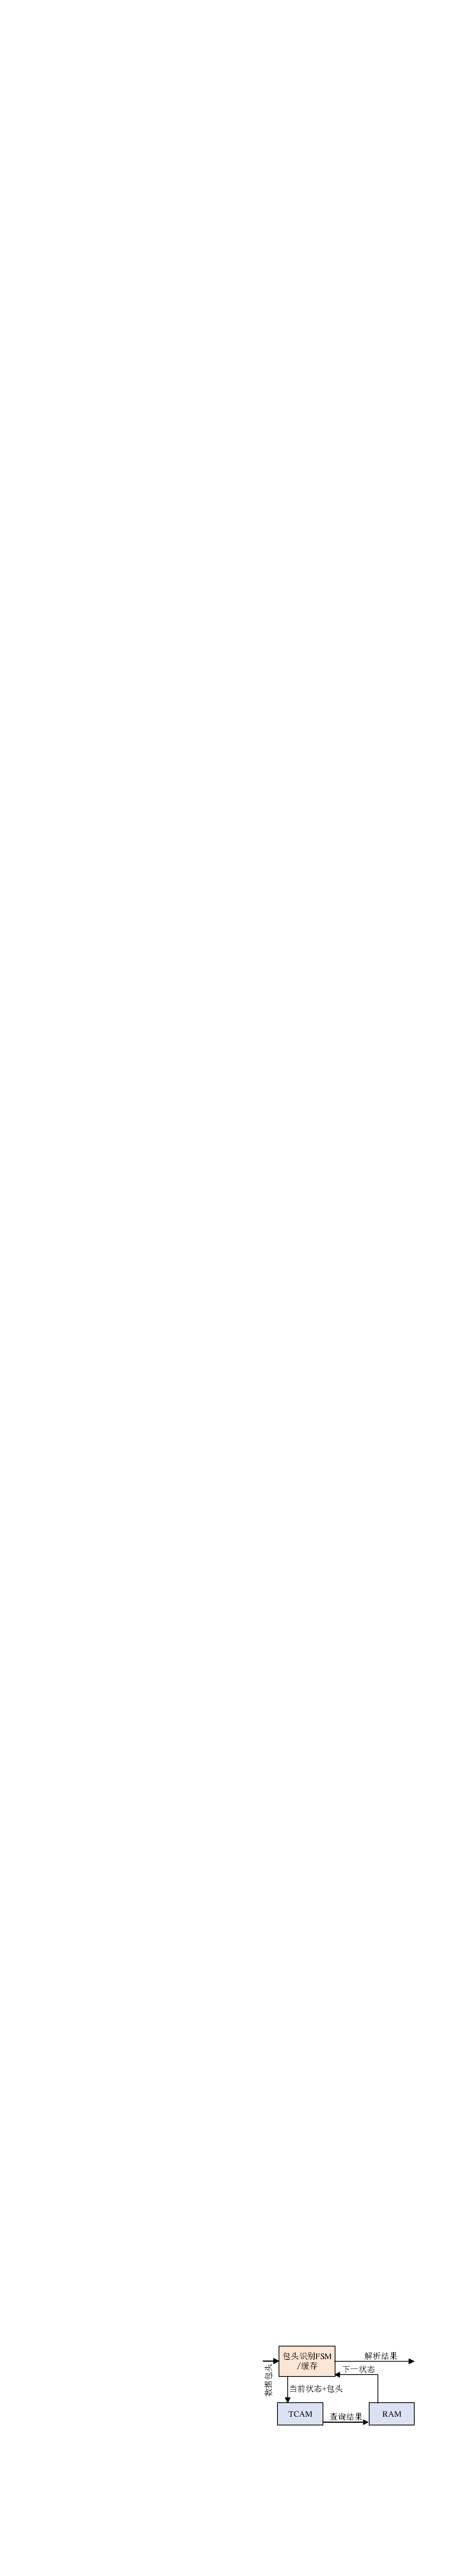
\includegraphics[scale=1]{progparser.pdf}
		\caption{基于ASIC的可编程包头协议解析器架构} \label{fig:progparser}
	\end{minipage}
\end{figure}



可编程包头解析器可以实现数据平面对新协议的可编程性。交换机中的查找表必须查找固定协议字段,所以每个交换机都会包括一个包头解析器,它能够标识当前数据包包头的协议名称。
如图\ref{fig:pktheader}所示,数据包是一组串行数据,从数据包的开始位置起,包头协议依次串行排列。每个协议段长度固定,每个协议末尾会有标识码标明下一个协议字段名称。本协议字段的长度一般都存储在协议字段内部。
包头中的协议字段是一种有向图关系,图的节点代表协议,向量字段代表转移关系。
一个包的包头不一定包含图中所有的节点和对应关系,但当数据包到来时,包头所包含的协议只能是有向图中的唯一一种路径。一般使用有限状态机(FSM)就可以提取出包头内的所有协议字段。FSM内部存储完整的图关系,只要按照图对应关系来给包头不同字段打上协议名称标签即可。


\BiSubsection{网络数据平面的可编程抽象方法}{Application and research status}\label{chap123}


{\hei 1)网络数据平面的全可编程抽象}


用智能网卡来卸载操作系统内的网络功能,以期望获得比CPU更好的效能,同时还可以兼顾网络设计中不断变化的革新需求。智能网卡也称可编程网卡,相比于普通网卡:智能网卡不但可以完成网卡最基本的作用(主机与网络间通信),还应该有如下特征:输入输出多队列、TCP卸载、流量整形、规则过滤、虚拟化等\citeup{shinde2013we}。从而增强一些通用场景下的网络性能:带宽扩容、优化QoS(Quality of Service,服务质量)、降低CPU利用率、降低通信时延等。

随着时间的推移,研究人员还发现如果能够将计算\citeup{costa2012camdoop,sapio2017network}、随路功能聚合\citeup{mai2014netagg,graham2016scalable}、缓存\citeup{liu2017incbricks}甚至AI\citeup{sanvito2018can,innetworknn}都卸载到网络上,有能力显著提高分布式应用的处理效率。
目前能够支持这种将更复杂计算卸载到网络中的网卡,都要求此智能网卡具有通用型的可编程能力。

基于网络处理器(Network Processor, NP)的数据平面,拥有完全的可编程能力。NP芯片内部一般包括基于硬件的拥塞控制、队列调度、QoS等协处理逻辑,还包括一组并行微码处理器。处理器按任务可分为核心处理器和转发引擎。处理器通过预先编制的微码来控制处理过程和内容。NP编程模式简单,一旦有新的技术或者需求出现,可以通过软件语义重新定义数据平面。值得注意的是NP中的众核一般使用数据平面专用精简指令集,为了达到节能与节约面积,像浮点运算等复杂的处理指令是不支持的。NP的每个内核处理性能一般较差,NP的高性能主要靠结合使用专用外挂电路。一旦处理的内容无法映射到专用电路,那么NP的性能会弱于通用软件。另外,NP编程开发门槛较高,NP运行软件无操作系统扶持。NP的代码移植性差,开发人员需要深入理解NP的处理模型。因此NP始终只在一些狭窄的领域空间内发挥作用。



基于FPGA的智能网卡拥有更为广阔的编程空间。FPGA内部有大量LUT门电路,以及分布式片上互联网络,基于此结构的FPGA可以实现任何客制化的逻辑电路。FPGA使用硬件描述语言开发(HDL),HDL不直接体现门电路的拼接方式而只是一种行为描述语言,从而屏蔽了底层细节。FPGA可以方便地移植程序,我们可以将HDL代码打包成IP核,只要按照规定好的输入输出接口位宽和时序就可以任意复用。在设计电路模组时,我们一般会使用标准的总线接口来连接不同的功能模块,以增强开发的灵活性。如今FPGA厂商也会在FPGA中加入专用功能电路来增加芯片集成度、增强FPGA的处理某些任务时的性能。如ARM核、分布式DSP核、PCIe收发器、分布式片上存储。

{\hei 2)专用领域系统的可编程抽象}



为应对日益复杂的网络功能的可编程扩展,网络功能可编程需求增加。可编程系统提供专用领域所特有的特性是提升网络功能开发效率的重要手段。高级的专用领域可编程抽象可以大大降低开发人员的编程难度。对于流匹配的可编程思想,SDN抽象出对流表配置的可编程\citeup{mckeown2008openflow},P4抽象出了对流定义的编程\citeup{p4}。
在数据中心内,网络的管理很复杂,需同时考虑流量控制,拥塞控制,访问控制,攻击探测等诸多网络功能的实现。



%{\hei 2)网络测量性能可扩展性不足}
网络测量是实现上文功能的底层核心方法,在性能方面有极大的需求\citeup{d2019survey}。流量控制,拥塞控制需要利用网络流量实时速度以及平均包大小等相关信息,访问控制和攻击探测也需要用到流触发的反馈测量机制\citeup{zhang2018adaptive}。基于被动触发的网络测量系统是一种典型的测量实现技术,测量过程一般分为1)捕获,2)统计,3)存储三大部分。这三点也是影响测量系统性能的关键因素。目前在可编程数据平面中,支持可编程实现的网络测量技术限制于以基于CPU或网络处理器的平台。其性能受到CPU架构访存与计算能力的制约,每核心单独处理统计量能力在10Gbps以内\citeup{estan2004building,tahaei2017multi,hu2013discount},相比于通用服务器目前上百Gbps的吞吐需求,显然存在比较明显的性能弱势。一方面由于目标流量数目庞大,基于CPU架构的快速缓存空间不足,多级存储结构带来复杂的更新机制并且受限于外存储的非连续地址访问速率(<1Mpps\citeup{linux2020andree,bernat2017performance,yang2016rethinking}),性能表现力不稳定\citeup{einziger2017tinylfu}。另一方面,CPU计算架构过于通用化,反而在处理简单重复的重任务时无法发挥优势,尤其针对流式数据处理,CPU无法建立起可编程的高效率的流水线结构,严重制约了网络功能处理能力的可扩展性\citeup{tone2009network}。


综上所述,现代高性能网络正在向软件定义化、数据平面可编程的方向发展。可编程网络架构设计的核心,是构建一种支持映射高层次控制逻辑的数据平面。本文主要以解决流表资源问题为基础,利用可编程硬件分别在网络中间节点、主机侧网络中构建了提升可编程性的方法,并形成一套完整的端到端系统。

\BiSection{论文研究内容与创新点}{Challenges}\label{chap13}



%\BiSubsection{论文研究内容与创新点}{Application and research status}\label{chap132}

%本文主要
本文以解决流表瓶颈资源问题为基础,研究在网络数据平面内如何利用可编程硬件来更灵活、更高效地支持多种类别的可编程抽象方法。针对高性能网络以及数据平面可编程领域内的三个挑战,本文利用可编程硬件分别在网络中间节点、主机侧网络中构建了能够同时提升设备性能以及灵活性的方法,最终构成一套完整的端到端网络系统。

\begin{figure}[!ht]
	\centering 
	\vspace{-1.5mm} 
	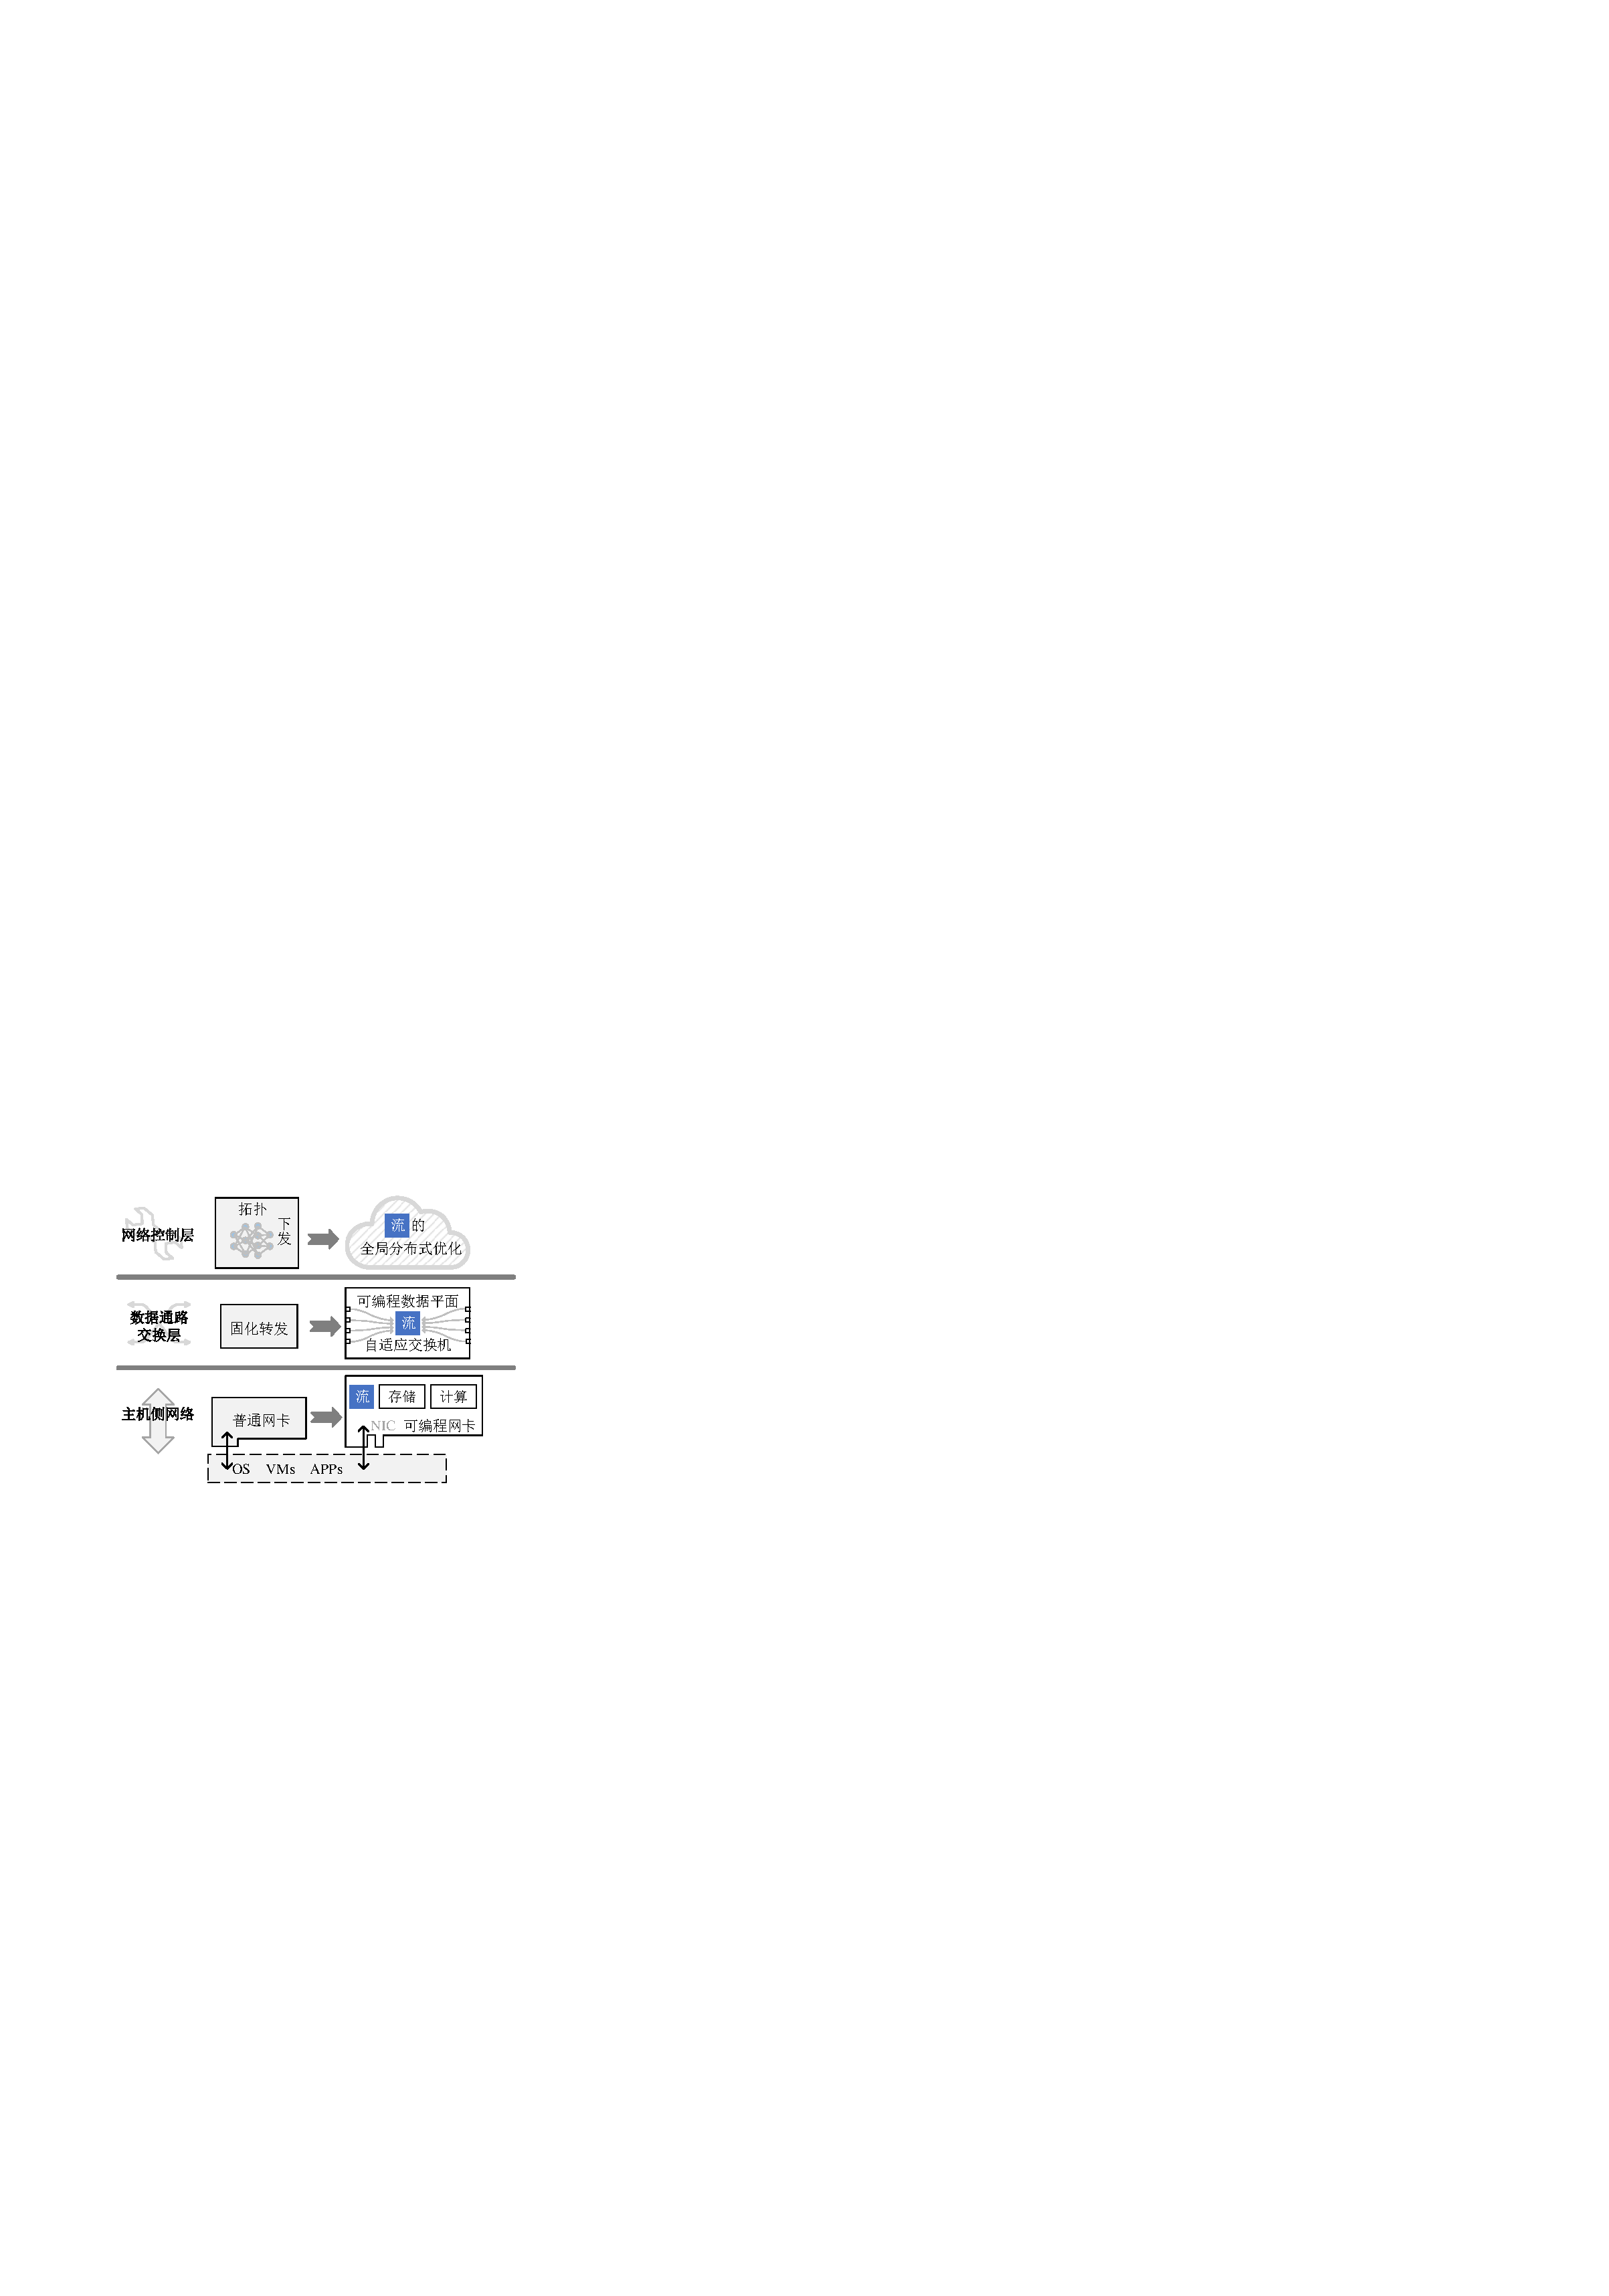
\includegraphics[scale=1]{proghardwarePDParcs.pdf}
	\caption{基于可编程硬件的SDN数据平面研究框架} \label{fig:proghardwarePDParcs}
\end{figure}

如图\ref{fig:proghardwarePDParcs}所示,本文从网络的三个层次出发,对可编程网络在每一个层次内做了改进。首先,流表是基于硬件的高性能数据包转发的核心资源,在研究内容一中利用软件定义网络控制平面高可配置性,对数据平面的流表资源进行了全局优化。其次,利用可编程硬件与交换芯片结合的异构结构,在研究内容二中设计一种自适应交换结构,优化数据平面网络节点的可编程能力。第三,针对主机侧网络中基于网络测量的网络功能,研究内容三提出了统一的软硬件结合编程抽象方法,利用硬件可编程网卡实现了高性能、高精度以及高效率的网络功能可编程系统。
%
%1.流表资源可扩展性研究。流表资源是各类数据平面可编程性的重要载体,为解决单个转发节点流表容量受限以及流表溢出后数据包处理性能严重下降的问题,本文提出了流表共享机制(FTS)。FTS通过与邻居节点建立流表共享机制,来提升整体流表资源的动态利用率,同时为无法建立流表项的流量设置基于离线转发策略的组表转发方式。在流表溢出的情况下,跟传统OpenFlow协议相比,使OpenFlow交换机转发RTT延迟和安全通道控制报文风暴数量的优化均达到至少2个数量级。
%
%2.可编程硬件使能网络中间节点的自适应计算能力。针对高性能网络转发设备可编程灵活性差的问题,本文提出了一种自适应交换的新型转发体系结构(AS),利用高性能的转发芯片与可编程硬件有机结合形成异构体,以及一套高资源利用率的并行流水线、流表分配优化算法,使AS系统在满足全可编程灵活性的条件下,与单纯可编程硬件的数据平面相比,将数据包处理性能提升120倍以上。
%
%3.端侧网络的领域内可编程研究。网络测量是众多网络功能的基础,针对目前其缺乏统一的编程抽象,本文提出了一套基于智能网卡的硬件流水线系统,包括数据包捕获功能、测量系统和发送引擎。本文将测量系统的可编程性抽象为基础的包个数统计和数据量缩统计方法。通过软件配置的方式,令系统硬件支持高性能的网络安全、访问控制、拥塞探测、流量控制等多种场景。同时利用基于硬件的存储压缩算法,在节约38\%FPGA片上存储空间情况下,相比基于软件的处理方式系统吞吐率提升8倍、能耗缩小为之前的十分之一。
%\BiSection{论文的组织结构安排}{Reasearch Contributions}\label{chap14}
具体研究内容概况如下:

{\hei 研究内容一:软件定义网络内交换机硬件流表可扩展性研究}

{\hei 本文从SDN网络全局视野出发,着手解决流表资源匮乏的问题。}由可编程网卡和交换机组成的数据平面内,流表资源是提升设备性能的核心,网络数据包的转发动作依赖于数据平面内查找表的匹配结果,在此基础上交换机内还增加了多种匹配域、多级流表结构,绝大多数平台中都视转发表为最核心以及成本占用最大的模块,软件定义网络(SDN)架构下亦是如此。
基于硬件的高性能TCAM\citeup{katta2014infinite}(三态内容地址查找表)拥有单周期流水、掩码匹配等优秀性能,但昂贵的价格使得用户无法购置容量足够大的表\citeup{kuzniar2015you},因此交换机内极易发生流表溢出的现象。
以OpenFlow协议为代表,一般规定控制器与交换机之间流表安装流程为Reactive模型:交换机收到一条新流首先会上报控制器,随后控制器计算路径并下发流表到数据平面设备。当发生流表溢出现象时,由于Reactive模型需要频繁更替活跃流表内容,这会进一步直接引发控制平面和数据平面之间安全通道的消息风暴,否则会造成丢包或服务任务中断等异常现象。第一个研究内容下有两个子问题:如何在维持交换机中原有流表容量的前提下,缓解流表溢出所带来的危害?在保持SDN网络平面分离优点的条件下,如何利用其全局化优势高效利用网络设备资源?


{\hei 创新点:}本文分析不同的流量规模和特征,以及系统多模块之间的互联协议,提出一种转发设备节点之间的流表共享机制(Flow Table Sharing, FTS)。

1)为保障控制平面免于遭受大量突发服务请求,FTS实现了一种离线转发策略,同时减轻了安全通道的通信压力。实现了在流量突发的情形下,保证数据平面稳定性,降低SDN系统控制通道拥塞、失效风险,缓解流表溢出导致转发性能骤降的现象。

2)为保障数据平面流表资源充足,本文分析并修改了目前OpenFlow协议中有关Table-Miss(流表缺失状态)的处理过程,并修改了OpenFlow协议中关于未知数据包上报条件,在数据平面内利用交换机组表进行聚合转发,并且可以方便地退回现有规范。

本文论证了单纯依靠增加流表容量的方案,并不能使流表溢出的概率降低为零,并且能够容易回退、向下兼容现阶段的传统方案。FTS通过通过增强数据平面自主性等方法,在流表溢出的情况下,该方案和传统OpenFlow协议相比,使OpenFlow交换机转发RTT延迟和安全通道控制报文风暴数量的优化均达到至少2个数量级。



{\hei 研究内容二:可编程设备增强网络交换节点计算能力的研究}

{\hei 本文从网络数据平面处理器的底层设计出发,在现有的大规模集成电路设计能力的基础上,构建可行的网络处理器流水线模型。}由于新兴的内容应用(社交,虚拟/增强,混合现实)以及工业网络应用(移动性,大数据,机器学习)使得网络追求高的实时性、可扩展性。网络设备功能多样性随着数据中心、边缘设备的发展而壮大,因此学界对交换层、核心网场景下快速创建灵活解决方案的需求也愈发强烈。可编程数据平面交换机的三类典型设计架构但目前都存在缺陷:1)软件交换机性能普遍低下,2)基于ASIC的交换机无法拥有完全可编程性,3)基于FPGA的交换机资源有限,交换性能无法满足业界需求。本文研究内容首先提出一种新型的可编程网络数据平面,采用异构设计的思想,解决上述典型设计的缺陷。
因此本文第二个研究问题:如何设计一种同时兼顾转发性能和可编程能力的交换设备?如何利用现有设备优势,对其做最小改动以满足设计?如何实现高资源利用率、高灵活性的高性能硬件可编程数据平面设计方法?

{\hei 创新点:}本文提出一种高性能的数据平面可编程硬件架构,自适应交换结构(Adaptable Switch, AS)。

1)为同时增强AS架构的灵活性和吞吐性能,AS提出一种旁路数据处理流水线模式。通过FPGA与交换芯片联合设计的思想,AS架构可同时提供FPGA的高灵活性与交换芯片的强大性能。论文在前述硬件设计模型的基础上,继续研究硬件逻辑高度并行的性能大规模扩展方法。

2)为增强可编程硬件内的数据处理吞吐能力,AS架构设计了一种资源占用低的流量均衡式并行处理模型。

3)为增强AS架构控制平面的处理性能,本文设计了一种高效的启发式流表分配算法。AS架构解决了FPGA性能差与资源少的限制、增强了网络芯片的可编程能力,并且提出了一套部署在硬件上的高资源利用率的并行流水线和流表分配优化算法。

论文设计了ASIC面向可编程硬件的扩展接口。交换芯片将数据包头拆分并通过高速数据互联载体发送给FPGA,利用FPGA可重配特性实现完全可编程的包头处理。自适应交换系统在满足全可编程灵活性的条件下,与基于FPGA的数据平面相比,将数据包处理性能提升120倍以上\footnote{当前的研究中,主流全可编程目标平台性能约为60Gbps。}。

{\hei 研究内容三:端侧网络的领域内可编程研究}

{\hei 本文提出利用基于FPGA的智能网卡卸载操作系统内网络测量任务,通过软件配置的方式,令系统硬件支持高性能的网络安全、访问控制、拥塞探测、流量控制等多种场景。}目前可编程网络领域缺乏对以上偏向底层的网络功能的统一抽象,开发人员需要独立实现功能细节,重新开发某些通用模块,耗费大量的人力物力。许多网络应用的基础是实现网络测量任务,本文将测量过程分解为三类子操作,1)捕获;2)统计分析;3)流量发送。捕获数据包时需要对每个数据包添加时间戳等数据记录工作,以供流量离线分析以及在线分析使用。在线统计分析对高性能和高实时性的特性要求极高。分析后的流量需要按原始流量顺序与速率再向网络接口发送回去。其中统计分析模块是可编程网络测量系统的核心模块,目前基于FPGA硬件可编程网卡同时提供了高性能收发和足够强大的灵活性已经可以满足主机侧网络的性能需求,为更复杂功能的卸载提供了有力支持\citeup{alveo250,netfpgaabout}。如何利用可编程网卡实现高精度、高性能保障和高能源效率的网络功能硬件卸载?提出测量功能可编程抽象、合理部署和划分任务是本文要解决的问题。

{\hei 创新点:}
网络测量是众多网络功能的基础,本文针对目前为了功能应用提出了统一的编程抽象方法。

1)为提升网络功能的编程灵活性,本文将针对网络测量领域的编程方式抽象为统计、触发模型。上层软件通过灵活调用测量数据来做更高层次的网络测量应用,令系统硬件适用于高性能的网络安全、访问控制、流量控制、拥塞探测等多种场景。

2)为增强终端可编程网络节点的性能,本文本文提出了一套基于智能网卡的硬件流水线系统,包括数据包捕获功能、测量系统和发送引擎。本文将其中测量系统操作抽象为基础的包个数统计和数据量缩统计方法。

3)为增基于测量的可编程网络抽象的可用性,本文本文提出一种基于硬件的存储压缩的无偏估计算法,在节约38\%的硬件存储空间情况下,相较于软件的处理方式系统吞吐率提升8倍、系统的处理能耗节约90\%。



如图\ref{fig:thesistree}所示,将本文的主要研究内容以及研究成果结构化地展示出来。


\begin{figure}[!ht]
	\centering 
	\vspace{-1.5mm}
	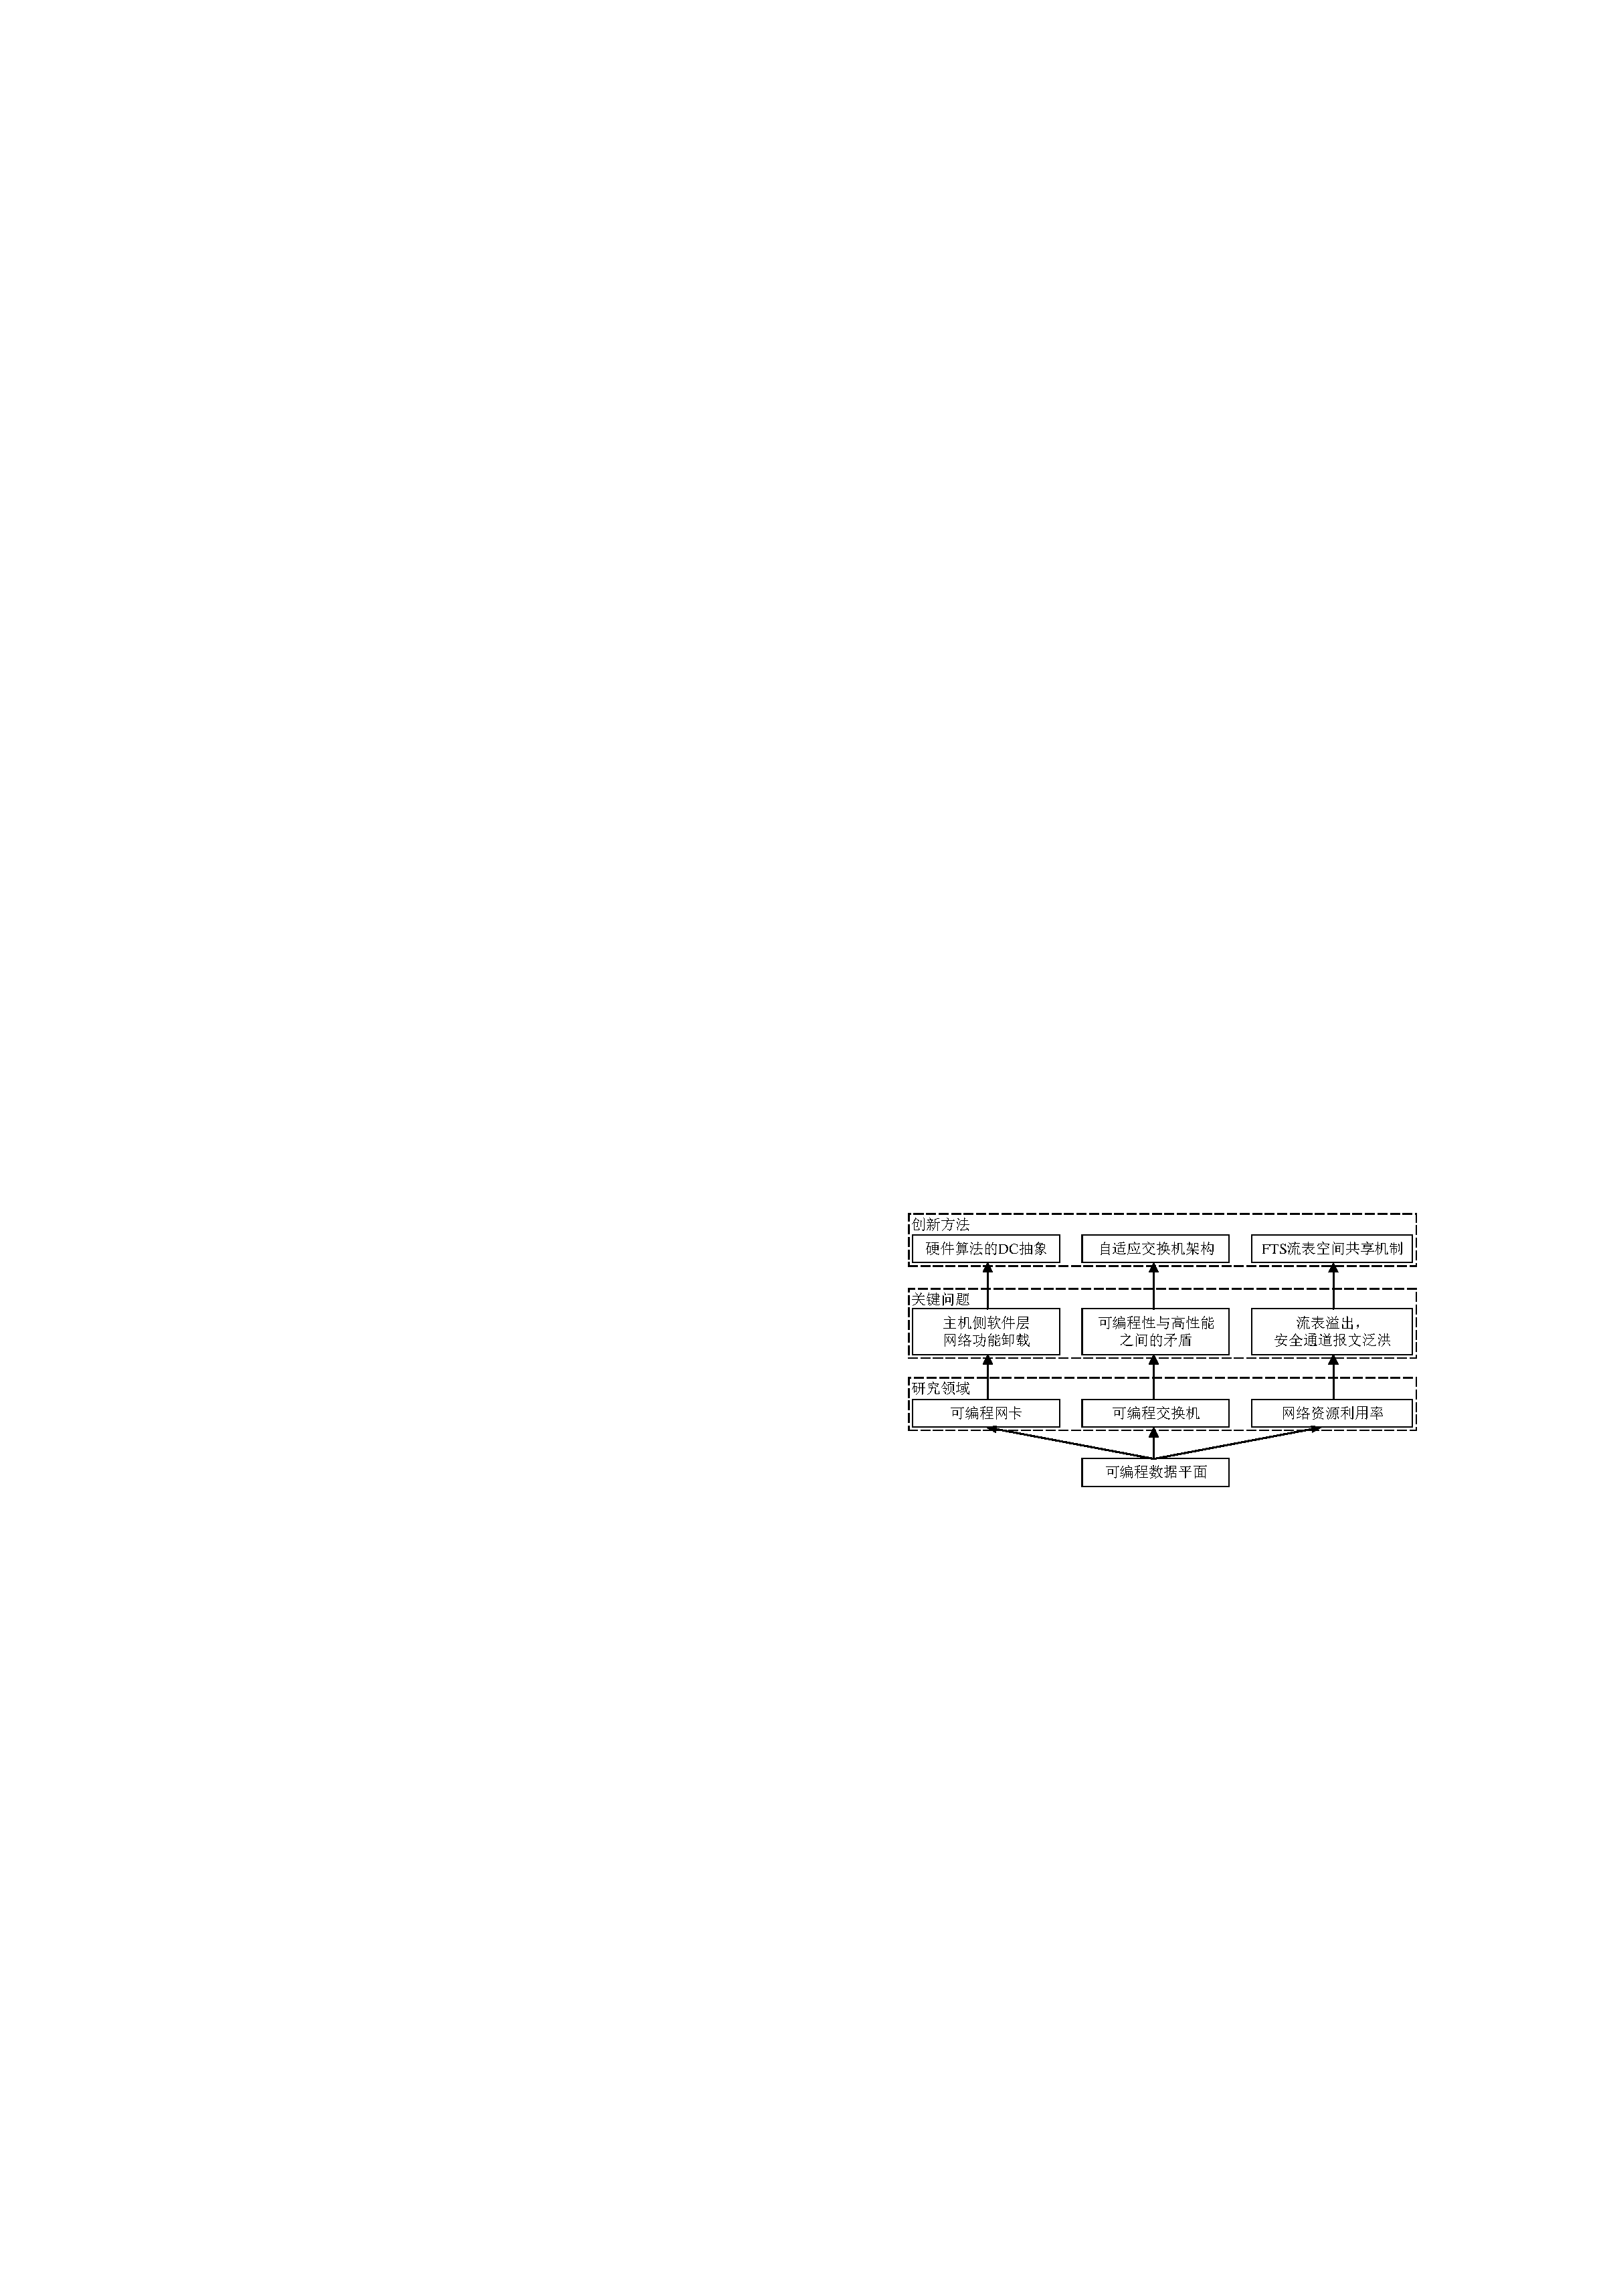
\includegraphics[scale=1]{thesistree.pdf}
	\caption{论文主要研究内容以及成果} \label{fig:thesistree}
\end{figure}



%本文提出一种针对网络测量领域的可编程智能网卡。将网络功能抽象为对全网流量的统计与触发,这种结构能够支持基于测量技术的广泛的网络应用:安防应用,访问控制,拥塞控制等。并且在硬件设计中,将网卡流水线抽象为三种操作,1)捕获,流量捕获下来可以做离线分析或在线实时分析;2)在线分析,将流的统计抽象为对每个流字节大小和包数目的统计,同时可计算并推导出其他丰富的测量指标,并且利用了压缩算法解决硬件高速缓存资源短缺的问题;3)发送引擎,将做完统计与测量的流量发送回网络,其中包括了原始流量,也可以发送合成后的主动探针流量。

%本文提出一种适用于网络功能硬件卸载的抽象模型:流式计算模型(DATA—COMPUTING, DC抽象)。根据DC抽象,分离软件中适用于硬件加速的繁杂计算,使原本经X86计算架构需要频繁访存的任务,转换到硬件中做流水线式流计算,可在不影响功能的前提下,释放CPU资源、扩展性能、提升系统效率。论文在可编程硬件的网卡中实现了更高精度、更高性能、资源利用率更好的流量捕获-统计-回放应用。实验证明利用可编程硬件能使原有软件性能效提升两个数量级、抖动降低4次方数量级、能源效率提升10倍。



\BiSection{论文组织结构}{Organization of the Thesis}\label{chap15}

论文共分为五个章节,具体组织结构安排如下:

第\ref{chap1}章为绪论,主要讨论研究背景、相关工作综述,分析可编程网络硬件的发展方向、目前研究所面临的挑战以及总述全文。本文接下来三章内容主要针对绪论提出的挑战而做出深入的研究。
%第\ref{sec:pdpintro}章为。

第\ref{chap5}章主要对网络数据平面内的流表资源做可扩展研究,提出一种全局优化方法来改善流表溢出带来的安全性风险。

第\ref{chap4}章论述一种FPGA与交换芯片相结合的异构网络数据平面硬件架构,令交换机系统拥有灵活的可编程能力的同时,处理吞吐性也能得到显著提升。

第\ref{chap3}章论提出了一种针对网络测量领域的可编程处理器,通过不同的软件调用,令系统硬件适用于高性能的网络安全、访问控制、流量控制、拥塞探测等多种场景。

第\ref{chap6}章总结全文工作,并展望未来研究方向。






%看一下,第二章的核心目的,再修改修改,增添一些画龙点睛的语段。参考李昊杨骥的完整版。
































%-----------------------------------------------------------------------------------------
%\BiSection{为什么用 \LaTeX}{Why}
%
%虽然论文排版是一项基本技能,但是从实际情况看,同学们经常被各种格式整得晕头转向。加之 Word 排版不够美观,版本管理麻烦,排版效率低下,因此开发 \LaTeX{} 论文模板非常重要。国际上许多著名的出版机构和学术期刊都有自己的 \LaTeX{} 模板,国内外许多高效也有自己的硕博论文 \LaTeX{} 模板。事实上,\LaTeX{} 已经成为科技出版行业的国际标准,特别是数学、物理、计算机和电子信息学科。
%
%采用 \LaTeX{} 排版主要有以下优点:
%\begin{enumerate}
%	\item 排版质量高:主要体现在对版面尺寸的严格控制,对字距、行距和段距等间距的松紧适度掌握,对数学公式的精细设计,对插图和表格的灵活处理,对代码和算法的优美呈现,等等。
%	\item 安全稳定:自发布以来 \TeX{} 和 \LaTeX{} 没有发现系统漏洞,不会出现死机或者系统崩溃而导致编写的内容来不及保存。
%	\item 灵活方便:\LaTeX{} 的源文件是纯文本文件,文件大小比 Word 小很多,不会因为文容的增加而导致文档打开、编辑、保存和关闭等操作变慢。因为 \LaTeX{} 在编译时才将所有源文件和图表汇总,故撰写内容时可以随意增删章节和图表。并且和大部分程序设计语言一样,\LaTeX{} 具有注释功能,作者可以在源文件任何地方添加注释,而不会影响最终生成的文档。
%	\item 格式和内容分离:\LaTeX{} 将文档格式和文档内容分开处理,作者只要选择合适的模板,就可专心致志地撰写文档内容,文档的格式细节则由 \LaTeX{} 模板统一规划设置。特别是文献管理能力非常强大,这给撰写像博士论文一样需要大量引用参考文献的文档提供了很大便利。
%	\item 免费开源:\LaTeX{} 软件完全免费,源代码也全部公开,并且相应的配套软件也都采用开源的方式。
%\end{enumerate}
%
%无论你是因为羡慕 \LaTeX{} 漂亮的输出结果,还是因为要给学术期刊投稿而被逼上梁山,都不得不面对这样一个事实:\LaTeX{} 是一种并不简单的排版软件,不可能只点点鼠标就弄好一篇漂亮的文章。还得拿出点搞研究的精神,通过不断练习,才能编排出整齐漂亮的论文。一旦你掌握了如何使用 \LaTeX{} 撰写出精美漂亮的论文时,你会发现你的决定是明智的,你的投入是值得的。
%
%%=========================================================================================
%\BiSection{怎样用 \LaTeX}{How} 
%
%本模板在 Windows + TeXLive2016 + Texsdudio 平台下开发,采用 XeLaTex 编译。虽然之前也开发过一个基于 CTeX 的模板,但是经过多方面比较发现 TeXLive+XeLaTex 处理中文更好,所以基于 CTeX 的模板没有共享。
%
%{\color{red}本模板不能在 CTeX 软件下使用,必须采用 TeXLive,并且编译方式是 XeLaTeX。TeXLive 每年更新一个版本,我用的是 TeXLive2016。文本编辑器可以根据自己的喜好选用,我用的是 Texsdudio,这款开源软件非常不错,推荐大家使用。}
%
%本模板的源文件通过主目录下的 main.tex 统一管理,setup 文件夹中存放格式定义和封面、摘要、目录等内容,body 文件夹中存放论文正文章节的源文件,appendix 文件夹中存放附录、致谢和声明等内容。
%
%本模板只提供论文的格式定义,不提供 \LaTeX{} 的详细使用方法。%所以只回复和论文格式相关的问题,不解答具体的排版方法和技巧。
%因为 \LaTeX{} 的资源非常丰富,大家可以在网上查找资料和并参与讨论,这样学习效率更高。我关注的两个网站是:\url{http://bbs.ctex.org/forum.php} 和 \url{http://www.latexstudio.net};参考的两本书是 ``The Not So Short Introduction to \LaTeXe'' 和 ``LaTeX2e完全学习手册''。
